% 5 to 10 pages
% talk about the experimentation
% adequacy, efficiency, productiveness, effectiveness
% (choose your criteria, state them clearly and justify them)
% be careful that you are using a fair measure, and that you are
% actually measuring what you claim to be measuring
% if comparing with previous techniques those techniques
% must be described in Chapter 2
% be honest in evaluation
% admit weaknesses

\section{Introduction}

\section{Experiment}


\section{Participants}
Data were recorded from 15 male and 1 female University students, aged between 18 and 32 (M = 25.00, SD = 3.875). As part of the experiment procedure demographic data were collected with special respect to the suggestions made by ~\cite{?}. Of the participants 94.1\% were right-handed. 41.2\% of participants rated their computer skills as Advanced while the rest of 58.8\% rated their skills as Intermediate. 35.3\% of participants have described themselves playing video games every day, while 41.2\% of them described themselves playing video games a few times per week and 17\% have been playing video games a few times per month and the rest of 5.9\% have been playing video games a few times per year. All participants have used PC as gaming system while 76.48\% of them also have used at least one of the four popular console platforms (XBox360, PS3, PS2, Wii) for gaming. All of participants had at least some experience with 3D shooting games like First Person Shooters. 47.1\% have described themselves playing 3D shooting games many times, while another 41.2\% described themselves as experts in 3D shooting games; Only a total of 11.8\% had limited or intermediate experience with 3D shooting games. Among the participants only 5.9\% had intermediate experience in using mouse in games, 35.3\% of them declared using mouse in games for many times and other 58.8\% of them described themselves as experts in doing that.

\section{Design}

A four condition (standard, player, NPC, environment) play session was employed to evaluate performance and excitement as dependent variables. The order 4 Latin square used to permute conditions between participants was as the following:

\centerline{a b c d}
\centerline{b c d a}
\centerline{c d a b}
\centerline{d a b c}

%%%%%%%%% nasty
at the start of the play session, they were required to press one of the four buttons on the entrance ramp labeled 1 to 4, and when any one of these buttons were pressed, the Affect engine started calibrating players signals for 60 seconds, during the calibration mode, no adjustment to any of game parameters is applied, no matter which condition is being played. After the one minute of calibration the system decides the standard range of signal for player's excitement value. After that except for the condition number 1 which is the no adaptation mode, the captured excitement value is normalized in the calibrated player range of excitement into a value between 0 and 1, and this value is then used to adjust the game parameters, this process of capturing, adjusting and applying the signal value would continue for 3 minutes until the next cycle of calibrating and adjustment starts. The player is required to play every condition for at least 5 minutes to ensure capturing of a complete cycle of calibrating and adjustment. After playing each condition, the player is asked to rest for 7 minutes, during this time the player is asked to fill out between condition questionnaires, which tries to ask the participant to self-estimate his affect level. The Player Mode is labeled as condition number 2, the NPC mode is labeled as condition number 3 and the Environment mode is labeled as condition number 4. From the 17 participants in this study, one has been lacking adequate level of expertise and therefore was unable to continue doing the required tasks at the expected level and therefore his results was not usable for this study. The image of signal values for this participant is depicted at the following:
%%%%%%%%% nasty

\section{Procedure}

The experiment was piloted with six participants (2 female). Pilot participants were selected from the Interaction Lab at the University of Saskatchewan, their comments on different mechanisms and online questionnaires of the experiment were reviewed to make participant more comfortable and less intervened during the experiment. Also pilot participants physiological data was recorded to confirm the functionality of the system during the experiment.

All experiments were conducted on weekdays, with the first slot beginning at 11:00h and the last ending at 18:30h. Participants were contacted to choose their preferred time slots while general time for one experimental session was 1:30 hours with setup and cleanup. Participants were invited to a laboratory, after a brief introduction of the experimental procedure, and becoming aware of the data being collected during the session, they were asked to fill out and sign informed consent form, this was the only paper form used during the experiment. Then the GSR sensors were attached to participant's hand.

Attached GSR sensors wired to the signal decoder brings limitations for participants while moving and using their hand. To diminish noisy signals and make participants feel comfortable under these limitations, the GSR sensors were attached to the hand that was handling the mouse during the game. While fingers dealing with mouse were quite steady compared to the other hand handling the keyboard, those fingers used to press the left and right mouse buttons were usually most comfortable ones for attaching GSR sensors. Some participants used index and middle fingers to press mouse buttons and others used index and ring fingers to do that \ref{fig:gsr-attached}.

\img
{Attaching GSR sensors}
{GSR sensors attached to index and middle finger of participant's right hand}
{gsr-attached.jpg}
{gsr-attached}

Having GSR sensors attached, participants were seated in a comfortable office chair, which was adjusted according to their individual height. They were then led to fill out the initial game demographic questionnaire. To keep GSR sensors attached during the experiment, all questionnaires after attaching GSR sensors were filled out using mouse and the same computer system. After the demographic questionnaire, participants were asked to self-assess their arousal, valence and dominance level using the self assessment manikin (SAM) questionnaire ~\cite{?}. Filling initial questionnaires after attaching GSR sensors was meant to give enough time (approximately 5 minutes) to the participant to get used to the sensors before playing the game. Participants then have been taken to a tour in the game. Different game mechanics were shown to them, and they were given about 1 minute, dependent to their experience, to make themselves comfortable with it. Some participants didn't need this time due to prior experience and asked to skip that. Then, participants played four different game conditions described before. Participants were not told about the differences between conditions. Each game condition was set to take 5 minutes. After each condition, participants were asked to write their comments about particular changes they noticed under that condition and its effect on their gameplay. Then they were asked to filled out the intrinsic motivation inventory (IMI) questionnaire, the player experience of need satisfaction (PENS) questionnaire and the game engagement questionnaire (GEQ) to rate their experience. Filling the questionnaires between conditions was done during the minimum 7 minutes of resting time before the next condition begins. The resting time was meant to restore players baseline signals. GSR sensors were recording players signals during both the play and the resting sessions from the beginning of the first condition to the ending of the last condition. After completion of the experiment, sensors were removed. Participants were debriefed and compensated \$15 Canadian dollars and escorted out of the lab.

%-----------------------------------------------------------
\begin{center}
\label{tbl:experiment-procedure}
\captionof{table}{Experiment procedure}
\begin{tabular}{+p{10cm}^r}
\bhline
\rowstyle{\bfseries}
Activity                                         & min. \\
\hline
Greetings, Consent form                          & ~2   \\
Installation of physiological sensors, a short description about the \newline
procedure and starting questionnaires            & ~3   \\
Introducing the game mechanics and a little practice if \newline
needed                                           & ~2   \\
Game condition a                                 & 5    \\
Condition questionnaire a                        & 7    \\
Game condition b                                 & 5    \\
Condition questionnaire b                        & 7    \\
Game condition c                                 & 5    \\
Condition questionnaire c                        & 7    \\
Game condition d                                 & 5    \\
Condition questionnaire d                        & 7    \\
Semi-structured post-game interview, debriefing  & ~5   \\ 
\rowstyle{\bfseries}
Total                                            & ~60  \\
\bhline
\end{tabular}
\end{center}
%-----------------------------------------------------------

\section{Materials and Measures}
\subsection{GSR}

\subsection{Subjective Measurements}

Participants were assessing their experience under different conditions, using four online questionnaires. FluidSurveys was used to host the questionnaires.

\paragraph{Self-Assessment Manikin}

After each condition participants were asked to rate the condition using 5-point Self-Assessment Manikin (SAM) \cite{bradley1994measuring} scale for arousal, valence and dominance. \textregistered FluidSurveys Multiple Choice widget was modified to include the SAM scales. Figure ~\ref{fig:sam} shows the arousal, valence and dominance scales used.

\begin{figure}[h!]
  \caption[Self-assessment manikin]
  {Self-assessment manikin for arousal, valence and dominance used after each condition and before the first condition}
  \centering
  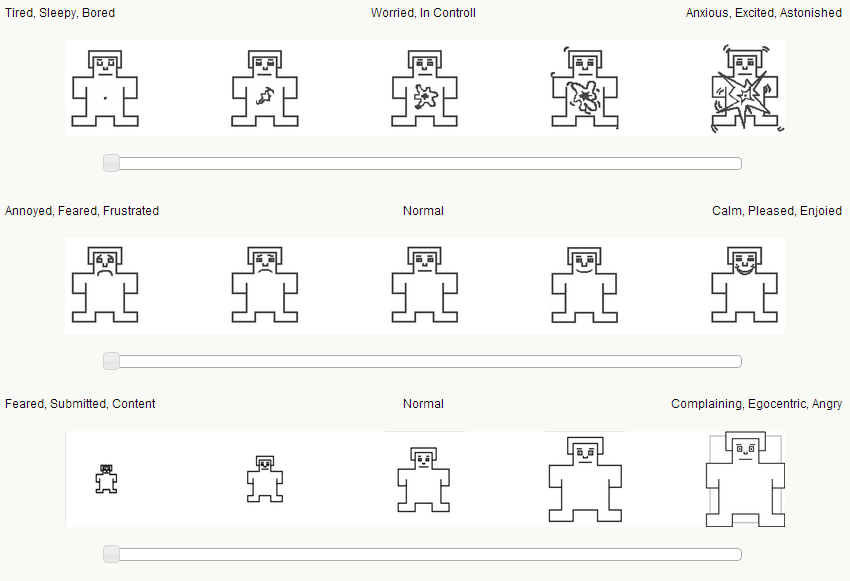
\includegraphics[width=0.7\textwidth]{images/sam.png}
  \label{fig:sam}
\end{figure}

\paragraph{Intrinsic Motivation Inventory}

Different components of game experience were measured using the Intrinsic Motivation Inventory questionnaire \cite{?}. It combines several game-related subjective measurement dimensions: interest/enjoyment, perceived competence, effort and felt pressure and tension while playing the game. Each one of these components consists of ?? question items (e.g., ``While playing, I was thinking about how much I enjoyed it'' is a interest/enjoyment component item). Question items were shown in a randomized order every time the page was viewed. Each question item consists of a statement on a five-point scale ranging from 1 (strongly disagreeing with the statement) to 5 (strongly agreeing with the statement). The questionnaire was developed based on survey studies \cite{?}.

\paragraph{Player Experience of Need Satisfaction}


\paragraph{Game Engagement Questionnaire}

%%%%%%%%%%%%%nasty%%%%%%%%%%%%%
An image of a regular participant signal values is depicted at
the following. In this image from left to right the light blue line
shows different conditions being played, and when the light blue
line is declining towards its base value, that is the period that
participant is asked to stop playing and instead relaxing and filling
out the questionnaires. The blue line is the normalized GSR signal
value of the participants which is used as an estimation of his
excitement level. The yellow green and pink lines are showing the
three different modes of Player, NPC and Environment parameters
being adapted

Following image is the GSR signal of players playing different
conditions from 1 to 4. From left to right the conditions are the
Default, Player, NPC and the Environment mode. This signals are all
based to an initial start value of 100, during the play experience,
some of them had gone bellow the start point and some other had risen
above that. Also the start time for each different condition is
shifted 500 seconds times the number of condition, from 0.

The following image is the average of GSR values for players in four
different conditions from left to right: Default, Player, NPC and
Environment modes
%%%%%%%%%%%%%nasty%%%%%%%%%%%%%

\section{Results}

% describe 16 participant's feedbacks and comments, and general ideas on how each one of them migh have experienced different situations through the game.

%-----------------------------------------------------------
\begin{center}
\label{tbl:players-stats}
\captionof{table}{Sixteen players with their performance, divided into four experience categories spread across all four conditions}
\begin{tabular}{+l^l^l^l^l}
\bhline
\rowstyle{\bfseries}
ID       &   Performance   &   Order   &   Experience   &   Condition \\
\hline
1        &   69            &   1       &   1            &   4 \\
2        &   74            &   1       &   2            &   1 \\
3        &   117           &   1       &   3            &   2 \\
4        &   106           &   1       &   4            &   3 \\
5        &   42            &   2       &   1            &   1 \\
6        &   86            &   2       &   2            &   2 \\
7        &   67            &   2       &   3            &   3 \\
8        &   118           &   2       &   4            &   4 \\
9        &   13            &   3       &   1            &   3 \\
10       &   106           &   3       &   2            &   4 \\
11       &   98            &   3       &   3            &   1 \\
12       &   140           &   3       &   4            &   2 \\
13       &   66            &   4       &   1            &   2 \\
14       &   58            &   4       &   2            &   3 \\
15       &   110           &   4       &   3            &   4 \\
16       &   140           &   4       &   4            &   1 \\
\bhline
\end{tabular}
\end{center}
%-----------------------------------------------------------

\img
{Normal Q-Q plot of players' performance}
{Normal Q-Q plot of players' performance}
{anova-qq-performance.pdf}
{players-qq-performance}

\img
{Plot of residuals vs. fitted values for players' performance}
{Plot of residuals vs. fitted values for players' performance}
{anova-residuals-vs-fitted-values-performance.pdf}
{residuals-vs-fitted-values-performance}


\img
{Normal Q-Q plot of players' excitement}
{Normal Q-Q plot of players' excitement}
{anova-qq-excitement.pdf}
{players-qq-excitement}

\img
{Plot of residuals vs. fitted values for players' excitement}
{Plot of residuals vs. fitted values for players' excitement}
{anova-residuals-vs-fitted-values-excitement.pdf}
{residuals-vs-fitted-values-excitement}

%-----------------------------------------------------------
\begin{center}
\label{tbl:unknown}
\captionof{table}{unknown}
\begin{tabular}{+l^l^l^l}
\bhline
\rowstyle{\bfseries}
Condition    & Mean estimation of performance   & Lower bound   & Upper bound \\
\hline
1            & 58.50                            &   45.60997    &   71.39003  \\
2            & 98.25                            &   85.35997    &   111.14003 \\
3            & 101.75                           &   88.85997    &   114.64003 \\
4            & 91.50                            &   78.60997    &   104.39003 \\
\bhline
\end{tabular}
\end{center}
%-----------------------------------------------------------

%%nasty from mahdi
In the above table we see that not all the means of performances of players across the conditions are equal. We use ANOVA to test whether the means are statistically equal. The p-value corresponding the hypothesis that all the means are equal is  0.01719944. Hence we come to realize that, at the level of 5\%, not all the means are equal. This may mean that manipulating the games may have changed the performances of the players. To see whether this assumption is true, we use Tukey's multiple comparison test. The results are as following:
%%nasty from mahdi

%-----------------------------------------------------------
\begin{center}
\label{tbl:unknown}
\captionof{table}{unknown}
\begin{tabular}{+l^l^l^l^l}
\bhline
\rowstyle{\bfseries}
Conditions' difference   &   Mean difference   &   Lower bound   &   Upper bound   &   P-value     \\
\hline
2-1                      &   39.75             &   10.787245     &   68.71276      &   0.0124504   \\
3-1                      &   43.25             &   14.287245     &   72.21276      &   0.0082819   \\
4-1                      &   33.00             &   4.037245      &   61.96276      &   0.0290272   \\
3-2                      &   3.50              &   -25.462755    &   32.46276      &   0.9732678   \\
4-2                      &   -6.75             &   -35.712755    &   22.21276      &   0.8492682   \\
4-3                      &   -10.25            &   -39.212755    &   18.71276      &   0.6351259   \\
\bhline
\end{tabular}
\end{center}
%-----------------------------------------------------------

% nasty from mahdi
The first three rows of the above table state that the players have significantly lower performance in the default condition, while the performances increase in the other three condition. The lower three rows of the table state that all the three conditions have the same influence on the default such that the performers have similar performances.

In this experiment, as mentioned earlier, we used Latin Square method. The blockings were Individuals' experiences and time order which were suspected to be nuisiance factors of this experiment. After apply the method, we gained the values:
F-ratio of run order= 1.2083 
F-ratio of experience= 29.0333.
The first value is small while the other is extremely large. We conclude that blocking the time order is not appropriate for such studies while experience had the potential to affect our results. In addition, we can say that different individuals' experiences resulted in different performances. This becomes more apparent when we note that if a player is more experienced than the other, s/he would have a better performance if the game is manipulated in order to make the game, sometimes, more challenging (condition 3) and sometimes of favour of the player (condition 2). The table below explains which condition is more suitable for different players with different game experiences:
% nasty from mahdi

%-----------------------------------------------------------
\begin{center}
\label{tbl:unknown}
\captionof{table}{unknown}
\begin{tabular}{+l^l^l^l^l}
\bhline
\rowstyle{\bfseries}
Experiences' difference   & Mean difference   & Lower bound   & Upper bound   & P-value     \\
\hline
2-1                       & 33.5              & 4.537245      & 62.46276      & 0.0271883   \\
3-1                       & 50.5              & 21.537245     & 79.46276      & 0.0037921   \\
4-1                       & 76.0              & 47.037245     & 104.96276     & 0.0004163   \\
3-2                       & 17.0              & -11.962755    & 45.96276      & 0.2745976   \\
4-2                       & 42.5              & 13.537245     & 71.46276      & 0.0090222   \\
4-3                       & 25.5              & -3.462755     & 54.46276      & 0.0812661   \\
\bhline
\end{tabular}
\end{center}
%-----------------------------------------------------------

\img
{Q-Q plot for excitement}
{Normal q-q plot for excitement}
{res-4.png}
{plot-excitement}

\img
{Plot of residuals vs. fitted values}
{Plot of residuals vs. fitted values}
{res-5.png}
{residuals-vs-fitted}

\img
{Plot of residuals vs. conditions}
{Plot of residuals vs. conditions}
{res-6.png}
{residuals-vs-conditions}

%-----------------------------------------------------------
\begin{center}
\label{tbl:unknown}
\captionof{table}{unknown}
\begin{tabular}{+l^l^l^l}
\bhline
\rowstyle{\bfseries}
Condition     &   Mean of GSR   &   Lower bound   &   Upper bound   \\
\hline
Default       &   -5.29680      &   -24.13608     &   13.54248      \\
Player        &   46.48590      &   27.64662      &   65.32518      \\
Zombie        &   26.95377      &   8.11450       &   45.79305      \\
Environment   &   22.99617      &   4.15690       &   41.83545      \\
\bhline
\end{tabular}
\end{center}
%-----------------------------------------------------------

% nasty from mahdi
p-value of the hypothesis that the excitement of players were the same across all the conditions= 0.06439932.
the ration for experience is 2.230153 which is small. So experience doesn't have an influence on players' excitement.
% nasty from mahdi
